\documentclass{report}

\input{preamble}
\input{macros}
\input{letterfonts}

\title{\Huge{MAM2000W}\\Inner Product Spaces}
\author{\huge{Alex Cristaudo}}
\date{}

\begin{document}

\maketitle
\newpage% or \cleardoublepage
% \pdfbookmark[<level>]{<title>}{<dest>}
\pdfbookmark[section]{\contentsname}{toc}
\tableofcontents
\pagebreak

\chapter{Inner Product Spaces}



\section{Inner Product Spaces}


\nt{
Inner Product is a generalisation of the dot product in $\mathbb{R}^2$ and $\mathbb{R}^3$
}
Properties of Dot Product:
\begin{itemize}
    \item $\mathbf{x} \cdot \mathbf{y} = \left( x_1, x_2, \ldots, x_n \right) \cdot \left( y_1, y_2, \ldots, y_n \right)  = x_1y_1 + x_2y_2 + \ldots + x_ny_n$ 
    \item $\mathbf{x} \cdot \mathbf{y} = \mathbf{y} \cdot \mathbf{x} $
    \item $\left( \mathbf{x} + \mathbf{y} \right) \cdot {\mathbf{z}} = \mathbf{x} \cdot \mathbf{z} + \mathbf{y} \cdot \mathbf{z} $
    \item $\left( \lambda \mathbf{x} \right) \cdot \mathbf{y} = \lambda \left( \mathbf{x} \cdot \mathbf{y} \right) $
    \item $\mathbf{x} \cdot \mathbf{x} \ge 0$ 
    \item $\mathbf{x} \cdot \mathbf{x} = 0 \iff \mathbf{x} = \mathbf{0}$
    
\end{itemize}

\nt{Inner Product or Inner Product Space?}
\dfn{Inner Product}{
Let $V$ be a vector space over  $\mathbb{R}$ or $\mathbb{C}$. \\ A function which assigns to any ordered pair $\mathbf{u}, \mathbf{v} \in V$ a scalar $ \langle \mathbf{u}, \mathbf{v} \rangle \in \mathbb{R}$ or $\mathbb{C}$ is an inner product on $V$ is the following hold
 \begin{itemize}
     \item $ \langle \mathbf{u}, \mathbf{v} \rangle = \overline{\langle \mathbf{v}, \mathbf{u} \rangle}$
    \item $ \langle \mathbf{u} + \mathbf{v}, \mathbf{w} \rangle = \langle \mathbf{u}, \mathbf{w} \rangle + \langle \mathbf{v}, \mathbf{w} \rangle$
    \item $\langle \lambda \mathbf{u}, \mathbf{v} \rangle = \lambda \langle \mathbf{u}, \mathbf{v} \rangle$
    \item $ \langle \mathbf{u}, \mathbf{u} \rangle \ge 0$ and $ \langle \mathbf{u}, \mathbf{u} \rangle = 0 \iff \mathbf{u} = \mathbf{0}$
\end{itemize}
}

\nt{
    If we deal with a real vector space, then condition 1 is: $\langle \mathbf{u},\mathbf{v} \rangle = \langle \mathbf{v}, \mathbf{u} \rangle$ \\
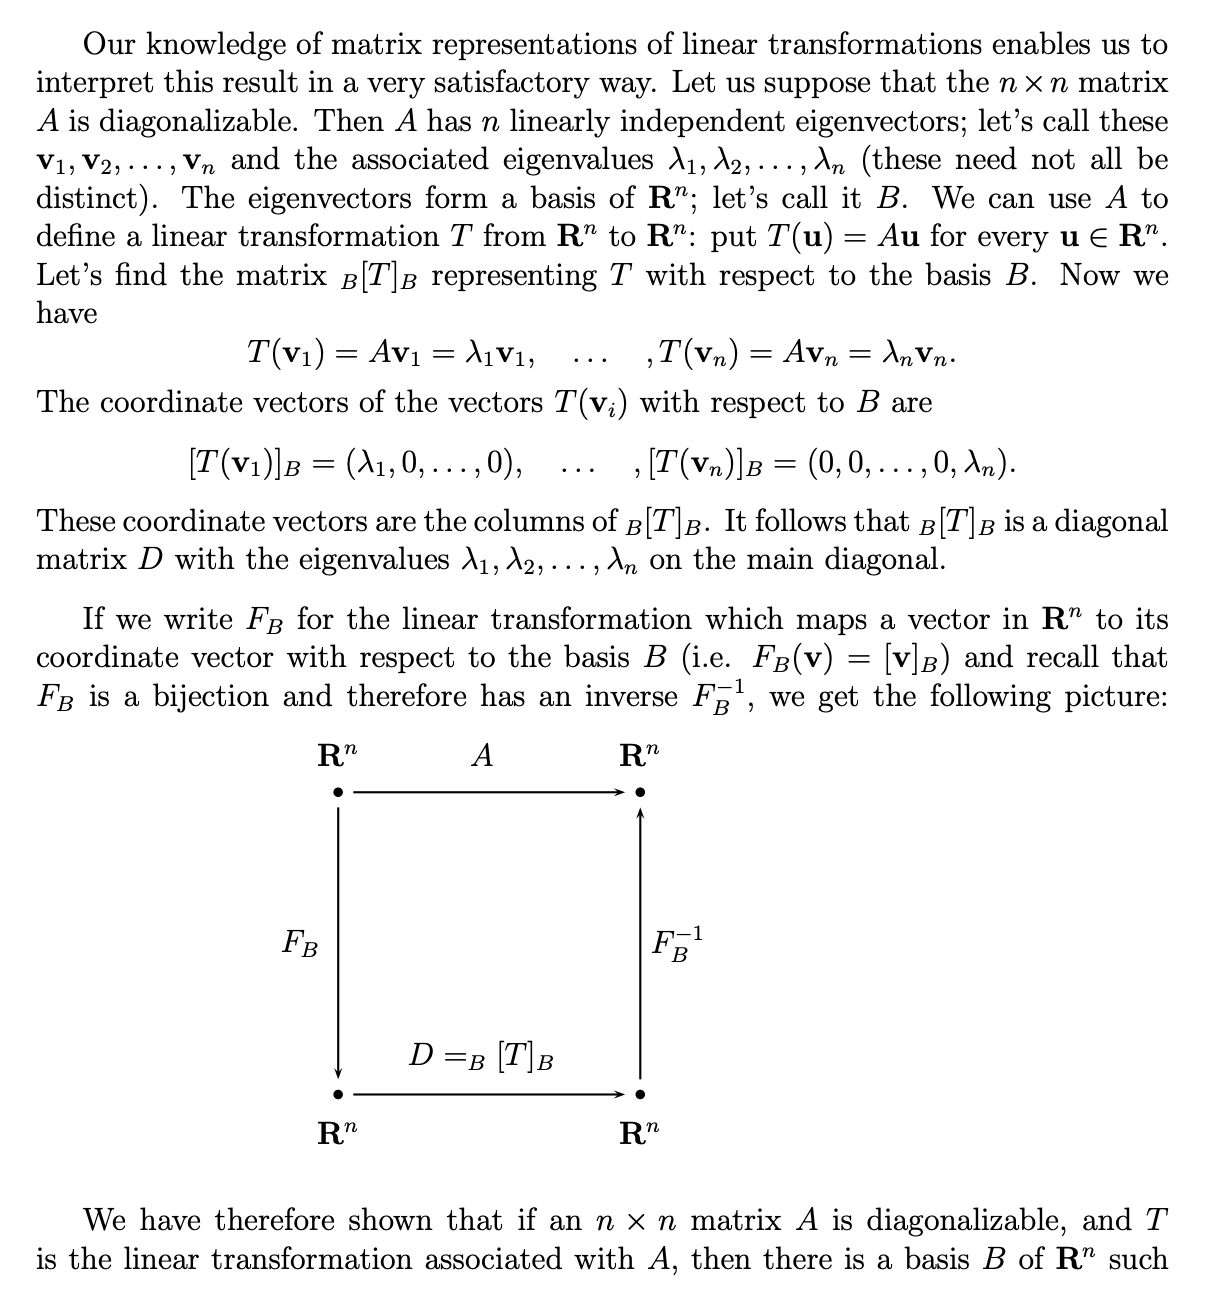
\includegraphics[scale = 0.8]{nt1}
}


\nt{
If there is an inner product defined on a vector space, we say the vector space is
equipped with an inner product. Any vector space equipped with an inner product is
called an inner product space.
}

\nt{
$ \langle \mathbf{u}, \mathbf{u} \rangle$ is real even if $\mathbf{u}$ is complex which is needed for comparison $\langle \mathbf{u}, \mathbf{u} \rangle \ge 0$ since we cannot compare with complex numbers
}

We now have a third operation on vector spaces: \\
$ \langle \rangle : V \times V \to \mathbb{R}$ or $\mathbb{C}$ 
\ex{}{
$V = \mathbb{R}^n$, then $\langle \mathbf{x}, \mathbf{y} \rangle = \mathbf{x} \cdot \mathbf{y}$
}
\ex{}{
    $V = C[0,1]$ (continuous ($C$ shows this) real-valued functions on  $[0,1]$ \\
    Then define  $\langle f,g \rangle = \int_{{0}}^{{1}} {f(x)g(x)} \: d{x}$ is an inner product
    \\ We have that \\
    \begin{itemize}
        \item $ \langle f, g \rangle = \langle g, f \rangle$
        \item  $ \langle f+g, h \rangle = \int_{{0}}^{{1}} {(f+g)(x)h(x)} \: d{x} \\ = \int_{{0}}^{{1}} {f(x)h(x)} \: d{x} + \int_{{0}}^{{1}} {g(x)h(x)} \: d{x} = \langle f,h \rangle + \langle g, h \rangle $
        
    \end{itemize}
}
\ex{}{
    $V = M_{m \times n}\left( \mathbb{R} \right) $. Defining $ \langle A,B \rangle = \mathrm{tr}\left( A^T \cdot B \right) $
    \\ Prove this is an inner product
}

\subsection{Properties of Inner Products}
\thm{}{
    \begin{enumerate}
        \item $\langle \mathbf{0}, \mathbf{u} \rangle = \langle \mathbf{u}, \mathbf{0} \rangle = 0$
            \nt{This is the zero in vector space}
        \item $\langle \mathbf{u}, \mathbf{v} + \mathbf{w} \rangle = \langle \mathbf{u}, \mathbf{v} \rangle + \langle \mathbf{u}, \mathbf{w} \rangle$
        \item $ \langle \mathbf{u}, \lambda \mathbf{v} \rangle = \overline{\lambda} \langle \mathbf{u}, \mathbf{v} \rangle$
        \item $\langle \mathbf{u} - \mathbf{v}, \mathbf{w} \rangle = \langle \mathbf{u}, \mathbf{w} \rangle - \langle \mathbf{v}, \mathbf{w} \rangle$
        \item $ \langle \mathbf{u}, \mathbf{v} - \mathbf{w} \rangle = \langle \mathbf{u}, \mathbf{v} \rangle - \langle \mathbf{u}, \mathbf{w} \rangle $
        \item If $\langle \mathbf{v}, \mathbf{w} \rangle = 0$ for all $\mathbf{w} \in V$, then $\mathbf{v} = \mathbf{0}$
    \end{enumerate}
}
\begin{myproof}
\begin{enumerate}
    \item $\langle \mathbf{0}, \mathbf{u} \rangle = \langle 0 \cdot \mathbf{u}, \mathbf{u} \rangle = 0 \langle \mathbf{u}, \mathbf{u} \rangle = \mathbf{0}$
    \item 
    \item $\langle \mathbf{u}, \lambda \mathbf{v} \rangle = \overline{{ \lambda }} \langle \mathbf{u}, \mathbf{v} \rangle$ 
        \nt{That is $ \lambda $ conjugate}
\end{enumerate}
\end{myproof}

\dfn{}{
Let $V$ be an inner product space and let  $\mathbf{v} \in V$. The norm of $\mathbf{v}$ (denoted by $ \vert \vert \mathbf{v}  \vert \vert $) is given by $\vert \vert \mathbf{v} \vert \vert = \sqrt{\langle \mathbf{v}, \mathbf{v} \rangle} $
}

\nt{In $\mathbb{R}^2$ and $\mathbb{R}^3$, the norm is the length of the vector. For higher dimensions, the norm is specified as the "size" (hard to visualise length in higher dimensions)}

\thm{}{
Let $\mathbf{u}$ and $\mathbf{v}$ be vectors in an inner product space. Then we have:
\begin{itemize}
    \item $\vert \langle \mathbf{u}, \mathbf{v} \rangle \vert \le \vert \vert \mathbf{u} \vert \vert \ \vert \vert \mathbf{v} \vert \vert$ \ \ \ \ (Cauchy-Schwarz inequality)
    \item $\vert \vert \mathbf{u} + \mathbf{v} \vert \vert \le \vert \vert \mathbf{u} \vert \vert + \vert \vert \mathbf{v} \vert \vert$ \ \ \ \ (Triangle inequality)
\end{itemize}
}

\begin{myproof}
    \begin{itemize}
        \item If either $\mathbf{u}$ or $\mathbf{v}$ is $\mathbf{0}$, then $\langle \mathbf{u}, \mathbf{v} \rangle$ and $\vert \vert \mathbf{u} \vert \vert \ \vert \vert \mathbf{v} \vert \vert$ are zero. So suppose $ \mathbf{u}$ and $\mathbf{v}$ are non-zero. Let $\mathbf{w} = \mathbf{u} - \lambda \mathbf{v}$ where $ \lambda $ is a scalar. We know that $ \langle \mathbf{w}, \mathbf{w} \rangle \ge 0 $ so
            \[
            \begin{aligned}
                0 & \le \langle \mathbf{u} - \lambda \mathbf{v}, \mathbf{u} - \lambda \mathbf{v} \rangle \\
                  &  = \langle \mathbf{u}, \mathbf{u} \rangle - \lambda \langle \mathbf{v}, \mathbf{u} \rangle - \overline{ \lambda } \langle \mathbf{u}, \mathbf{v} \rangle + \vert \lambda \vert ^2 \langle \mathbf{v}, \mathbf{v} \rangle \\
                   & = \langle \mathbf{u}, \mathbf{u} \rangle - \lambda \langle \mathbf{v}, \mathbf{u} \rangle - \overline{ \lambda  \langle \mathbf{u}, \mathbf{v} \rangle} + \vert \lambda \vert ^2 \langle \mathbf{v}, \mathbf{v} \rangle \\
                 & = \langle \mathbf{u}, \mathbf{u} \rangle - 2 \mathrm{Re}(\lambda \langle \mathbf{v}, \mathbf{u} \rangle) + \vert \lambda \vert ^2 \langle \mathbf{v}, \mathbf{v} \rangle \\
                 & = \vert \vert \mathbf{u} \vert \vert ^2 - 2 \mathrm{Re}(\lambda \langle \mathbf{v}, \mathbf{u} \rangle) + \vert \lambda \vert ^2 \ \vert \vert \mathbf{v} \vert \vert ^2 \\
            \end{aligned}
            \]
            Now let $ \lambda = \frac{\overline{ \langle \mathbf{v}, \mathbf{u} \rangle}}{\langle \mathbf{v}, \mathbf{v} \rangle}$. Then \\
            \[
            \begin{aligned}
                0  & \le \vert \vert \mathbf{u} \vert \vert ^2 - 2 \mathrm{Re} \bigg ( \frac{ \vert \langle \mathbf{v}, \mathbf{u} \rangle \vert ^2 }{\vert \vert \mathbf{v} \vert \vert ^2} \bigg ) + \frac{\vert \langle \mathbf{v}, \mathbf{u} \rangle \vert ^2}{\vert \vert \mathbf{v} \vert \vert ^4} \vert \vert \mathbf{v} \vert \vert ^2 \\
                 & = \vert \vert \mathbf{u} \vert \vert ^2 - \frac{\vert \langle \mathbf{v}, \mathbf{u} \rangle \vert ^2}{\vert \vert \mathbf{v} \vert \vert^2}
            \end{aligned}
            \]
        Thus we have
        \[
        \begin{aligned}
            0 \le \vert \vert \mathbf{u} \vert \vert ^2 \vert \vert \mathbf{v} \vert \vert ^2 - \vert \langle \mathbf{v}, \mathbf{u} \rangle \vert ^2  & \iff \vert \langle \mathbf{u}, \mathbf{v} \rangle \vert ^2 = \vert \langle \mathbf{v}, \mathbf{u} \rangle \vert ^2 \le \vert \vert \mathbf{u} \vert \vert ^2 \vert \vert \mathbf{v} \vert \vert ^2
        \end{aligned}
        \]
        Taking positive square roots gives the required answer
        \nt{Root function is increasing and one-to-one so this is true (not true that $x \le  x^2$, but true that $x^2 \le y^2 \implies \vert x \vert \le \vert y \vert$}
    \item By the Cauchy-Schwartz inequality, \\ 
\begin{center}
    $ \langle \mathbf{u}, \mathbf{v} \rangle \le \vert \langle \mathbf{u}, \mathbf{v} \rangle \vert \le \vert \vert \mathbf{u} \vert \vert \ \vert \vert \mathbf{v} \vert \vert$
\end{center}
Thus
\[
\begin{aligned}
    \vert \vert \mathbf{u} + \mathbf{v} \vert \vert ^2  & = \langle \mathbf{u} + \mathbf{v}, \mathbf{u} + \mathbf{v} \rangle \\
     &  = \langle \mathbf{u}, \mathbf{u} \rangle + 2 \langle \mathbf{u}, \mathbf{v} \rangle + \langle \mathbf{v}, \mathbf{v} \rangle \\
      & \le \vert \vert \mathbf{u} \vert \vert ^2 + 2 \vert \vert \mathbf{u} \vert \vert \ \vert \vert \mathbf{v} \vert \vert + \vert \vert \mathbf{v} \vert \vert ^2 \\
       & = \left( \vert \vert \mathbf{v} \vert \vert + \vert \vert \mathbf{v} \vert \vert \right)^2 
\end{aligned}
\]
Thus $\vert \vert \mathbf{u} + \mathbf{v} \vert \vert ^2 \le \left( \vert \vert \mathbf{u} \vert \vert + \vert \vert \mathbf{v} \vert \vert \right)^2 $ and taking positive square roots gives us the desired
result
\end{itemize}
\end{myproof}

\section{Orthogonality and Orthonormal Bases}

\nt{
We turn now to something you are already familiar with, that is, the idea of an angle
between vectors. In fact, the idea of an angle between vectors is not as important
in general vector spaces as it is in $\mathbb{R}^2 $ or $\mathbb{R}^3$
. What does remain of great importance
though, is the notion of perpendicularity or orthogonality. Recall from your first
year course that two vectors in $\mathbb{R}^2$ or $\mathbb{R}^3$ are perpendicular if their dot product is
zero. We extend this idea to any inner product space.
}

\dfn{}{
Let $\mathbf{u}$ and $\mathbf{v}$ be vectors in an inner product space $V$. We say  $\mathbf{u}$ and $\mathbf{v}$ are orthogonal if and only if $\langle \mathbf{u}, \mathbf{v} \rangle = 0$ (their inner product is 0). We say $\mathbf{u} \perp \mathbf{v} \iff \langle \mathbf{u}, \mathbf{v} \rangle = 0$
}

\ex{}{
    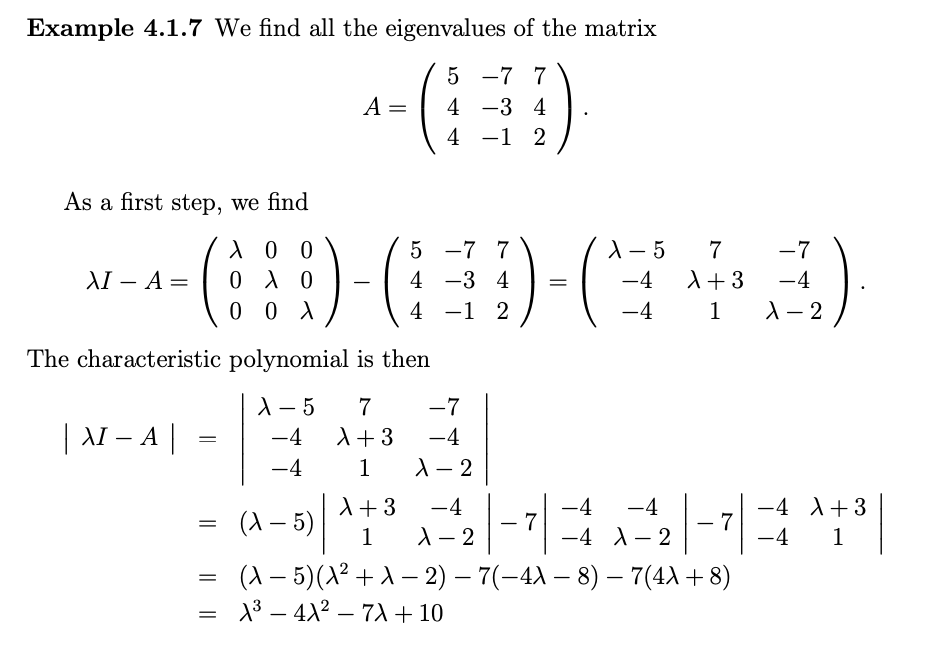
\includegraphics[scale = 0.9]{ex1}
}

\thm{}{
Let $\mathbf{u}$ and $\mathbf{v}$ be vectors in an inner product space $V$ such that  $\mathbf{u} \perp \mathbf{v}$. Then
\begin{center}
    $\vert \vert \mathbf{u} \vert \vert ^2 + \vert \vert \mathbf{v} \vert \vert^2 = \vert \vert \mathbf{u} + \mathbf{v} \vert \vert ^2 $
\end{center}
}
\begin{myproof}[]
    We have
    \[
    \begin{aligned}
        \vert \vert \mathbf{u} + \mathbf{v} \vert \vert ^2  & = \langle \mathbf{u} + \mathbf{v}, \mathbf{u} + \mathbf{v} \rangle \\
         & = \langle \mathbf{u}, \mathbf{u} \rangle + 2\langle \mathbf{u}, \mathbf{v} \rangle + \langle \mathbf{v}, \mathbf{v} \rangle \\
          & = \langle \mathbf{u}, \mathbf{u} \rangle + \langle \mathbf{v}, \mathbf{v} \rangle
           & = \vert \vert \mathbf{u} \vert \vert ^2 + \vert \vert \mathbf{v} \vert \vert ^2
    \end{aligned}
    \]
\end{myproof}

\dfn{}{
Let $S$ be a set of distinct vectors in an inner product space  $V$
 \begin{itemize}
    \item $S$ is said to be orthogonal if every pair of distinct vectors in the set  $S$ are orthogonal
    \item A vector  $\mathbf{v}$ is said to be normal if $ \vert \vert \mathbf{v} \vert \vert = 1$
    \item $S$ is orthonormal if  $S$ is orthogonal and each member of $S$ is normal
\end{itemize}
}

\nt{The standard basis $\{\left( 1,0,0 \right), \left( 0,1,0 \right), \left( 0,0,1 \right)   \}$ of $\mathbb{R}^3$ (and more generally the standard basis for $\mathbb{R}^n$) is particularly convenient to work with. This can be attributed
mainly to the fact that this basis forms an orthonormal set. Conversely, we’ll see that
in general orthogonal (and orthonormal) sets of vectors have many of the desirable
properties of the standard basis in $\mathbb{R}^n$}

\thm{}{
If $ \mathbf{v}_1, \mathbf{v}_2, \cdots, \mathbf{v}_{n}$ are non-zero orthogonal vectors, then they are linearly independent
}
\begin{myproof}[]
    Suppose $ \lambda_1, \lambda_2, \cdots, \lambda_{n}$ are scalars such that $ \lambda_1 \mathbf{v}_1 + \lambda _2 \mathbf{v}_2 + \cdots + \lambda_{n}\mathbf{v}_{n} = \mathbf{0}$\\ We wish to show each $ \lambda _i = 0$. Pick any $\mathbf{v}_i$, then \\
    \[
    \begin{aligned}
        0 = \langle \mathbf{0}, \mathbf{v}_i \rangle  & = \langle \left( \lambda_1 \mathbf{v}_1 + \lambda _2 \mathbf{v}_2 + \cdots + \lambda_{n}\mathbf{v}_{n} \right), \mathbf{v}_i \rangle \\
         & = \lambda_1 \langle \mathbf{v}_1, \mathbf{v}_i \rangle + \lambda _2 \langle \mathbf{v}_2, \mathbf{v}_i \rangle + \cdots + \lambda_{n} \langle \mathbf{v}_{n}, \mathbf{v}_i \rangle \\
          & = \lambda _i \langle \mathbf{v}_i , \mathbf{v}_i \rangle \left( \langle \mathbf{v}_j, \mathbf{v}_i \rangle = 0 \ \ i \ne j \right) 
    \end{aligned}
    \]
    but $\langle \mathbf{v}_i, \mathbf{v}_i \rangle \ne 0 \implies \lambda _i = 0$
\end{myproof}

\dfn{}{A basis $B$ for a vector space  $V$ is orthogonal if the set  $B$ is orthogonal; it is orthonormal if  $B$ is orthonormal}

\ex{}{
    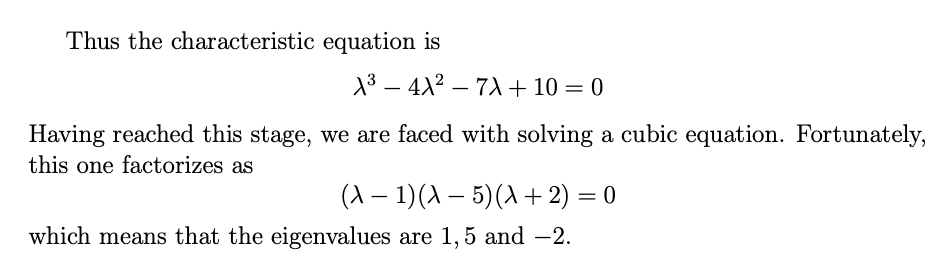
\includegraphics[scale = 0.9]{ex2}
}

We look now at an algorithm for transforming any (finite) basis of an inner
product space into an orthonormal basis. The fact that we can do this means that
any finite-dimensional inner product space space has an orthonormal basis. The
procedure we use is known as the Gram-Schmidt algorithm.

\thm{}{
Every (non-zero) finite-dimensional inner product space $V$ has an orthonormal basis
}
\begin{myproof}[]
    We do not prove this
\end{myproof}

The algorithm follows the following steps: \\
Let $B = \{ \mathbf{v}_1, \mathbf{v}_2, \cdots, \mathbf{v}_{n} \}$ be any basis for $V$. We give a rule for determining a set  $\{ \mathbf{u}_1, \mathbf{u}_2, \cdots, \mathbf{u}_{n} \}$ ($\mathbf{u}$ for unit) of orthonormal vectors (which must then be an orthonormal basis)
\\ \textbf{STEP 1: } $\mathbf{v}_1 \ne \mathbf{0}$ so we set $\mathbf{u}_1 = \frac{\mathbf{v}_1}{\vert \vert \mathbf{v}_1 \vert \vert}$. Then $\mathbf{u}_1$ is normal
\\ Recall the projection of $\mathbf{v}_2$ onto $\mathbf{u}_1$ is \\
\begin{center}
    $\frac{\langle \mathbf{v}_2, \mathbf{u}_1 \rangle}{\langle \mathbf{u}_1, \mathbf{u}_1 \rangle} \mathbf{u}_1 = \langle \mathbf{v}_2, \mathbf{u}_1 \rangle \mathbf{u}_1$
\end{center}
since $\vert \vert \mathbf{u}_1 = 1$, then
\begin{center}
    $\mathbf{w}_2 = \mathbf{v}_2 - \langle \mathbf{v}_2, \mathbf{u}_1 \rangle \mathbf{u}_1$
\end{center}
is orthogonal to $\mathbf{u}_1$. Also $\mathbf{w}_2$ is non-zero,  since if it were
zero, we would have a non-trivial linear combination of $\mathbf{v}_1$ and $\mathbf{v}_2$ yielding the zero
vector, which contradicts the linear independence
\\ We set $\mathbf{u}_2 = \frac{\mathbf{w}_2}{\vert \vert \mathbf{w}_2 \vert \vert}$
\\ \textbf{STEP 3: } The projections of $\mathbf{v}_3$ onto $\mathbf{u}_1$ and $\mathbf{u}_2 $ are respectively
\begin{center}
    $\langle \mathbf{v}_3, \mathbf{u}_1 \rangle \mathbf{u}_1$ and ${\langle \mathbf{v}_3, \mathbf{u}_2 \rangle \mathbf{u}_2}$\\    
\end{center}
    If we subtract these two projections from v3 the resulting vector, w3, will be orthogonal to both u1 and u2, but only because u1 and u2 are orthonormal. Let’s see
why:\\
\[
\begin{aligned}
    \langle \mathbf{w}_3, \mathbf{u}_1 \rangle  & = \langle \mathbf{v}_3 - \langle \mathbf{v}_3, \mathbf{u}_1 \rangle \mathbf{u}_1 - \langle \mathbf{v}_3, \mathbf{u}_2 \rangle \mathbf{u}_2, \mathbf{u}_1 \rangle \\
     & = \langle \mathbf{v}_3, \mathbf{u}_1 \rangle - \langle \mathbf{v}_3, \mathbf{u}_1 \rangle \langle \mathbf{u}_1, \mathbf{u}_1 \rangle - \langle \mathbf{v}_3, \mathbf{u}_2 \rangle \langle \mathbf{u}_2, \mathbf{u}_1 \rangle \\  & = 0
\end{aligned}
\]
The check for u2 is similar. Also w3 cannot be the zero vector because of the linear
independence of v1, v2 and v3. We set
\\ $\mathbf{u}_3 = \frac{\mathbf{w}_3}{\vert \vert \mathbf{w}_3 \vert \vert}$ 
\\ \textbf{STEPS 4 to $n$ : } Repeat as above with the obvious modifications
\\ The result is a set of n orthonormal vectors, which must be a basis for the original
space

\cor{}{
    With the notation above, for each $k, 1 \le k \le n$, the set  $\{\mathbf{u}_1, \ldots, \mathbf{u}_k\}$ spans the same subspace as the set $\{\mathbf{v}_1, \ldots, \mathbf{v}_k\}$
}

\ex{}{
    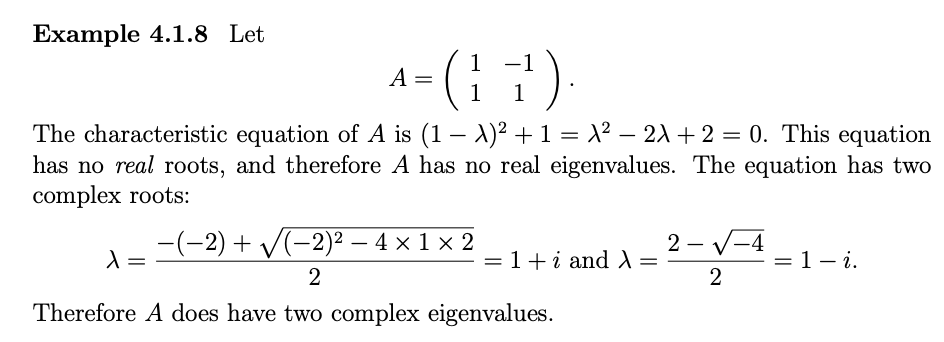
\includegraphics[scale = 0.9]{ex3}
}
\end{document}
